%%%%%%%%%%%%%%%%%%%%%%%%%%%%%%%%%%%%%%%%%%%%%%%%%%%%%%%%%%%%%%%%%%%%%
% Henriekes Mitschrieb vom 07.11.2013                               %
%%%%%%%%%%%%%%%%%%%%%%%%%%%%%%%%%%%%%%%%%%%%%%%%%%%%%%%%%%%%%%%%%%%%%
\chapter{Mannigfaltigkeiten und Simpizidkomplexe}
\section{Topologische Mannigfaltigkeiten}
\begin{definition}
    Sei $X$ ein topologischer Raum und $n \in \mdn$.
    \begin{enumerate}[label=(\alph*)]
        \item Eine $n$-dimensionale \textbf{Karte}\xindex{Karte} auf
              $X$ ist ein Paar $(U, \varphi)$, wobei $U \subseteq X$
              offen und $\varphi: U \rightarrow V$ Homöomorphismus
              von $U$ auf eine offene Teilmenge $V \subseteq \mdr^n$.
        \item Ein $n$-dimensionaler \textbf{Atlas}\xindex{Atlas} auf $X$ ist eine
              Familie $(U_i, \varphi_i)_{i \in I}$ von Karten auf $X$,
              sodass $\bigcup_{i \in I} U_i = X$.
        \item $X$ heißt (topologische) $n$-dimensionale \textbf{Mannigfaltigkeit}\xindex{Mannigfaltigkeit},
              wenn $X$ hausdorffsch ist, eine abzählbare Basis der 
              Topologie hat und ein $n$-dimensionalen Atlas besitzt.
    \end{enumerate}
\end{definition}

\begin{bemerkung}
    \begin{enumerate}[label=(\alph*)]
        \item Es gibt surjektive, stetige Abbildungen $[0,1] \rightarrow [0,1] \times [0,1]$
        \item Für $n \neq m$ sind $\mdr^n$ und $\mdr^m$ nicht homöomorph.
              Zum Beweis benutzt man den \enquote{Satz von der Gebietstreue} (Brouwer):

              Ist $U \subseteq \mdr^n$ offen und $f: U \rightarrow \mdr^n$
              stetig und injektiv, so ist $f(U)$ offen.

              Ist $n < m$ und $\mdr^m$ homöomorph zu $\mdr^n$, so wäre
              \[f:\mdr^n \rightarrow \mdr^m \rightarrow \mdr^n, \;\;\; (x_1, \dots, x_n) \mapsto (x_1, x_2, \dots, x_n, 0, \dots, 0)\]
              eine stetige injektive Abbildung. Also müsste $f(\mdr^n)$
              offen sein $\Rightarrow$ Widerspruch
    \end{enumerate}
\end{bemerkung}

\begin{beispiel}
    \begin{enumerate}[label=\arabic*)]
        \item Jede offene Teilmenge $U \subseteq \mdr^n$ ist eine 
              $n$-dimensionale Mannigfaltigkeit mit einem Atlas aus 
              einer Karte.
        \item $\mdc^n$ ist eine $2n$-dimensionale Mannigfaltigkeit
              mit einem Atlas aus einer Karte:
              \[(z_1, \dots, z_n) \mapsto (\operatorname{Re} z_1, \operatorname{Im}z_1, \dots, \operatorname{Re}z_n, \operatorname{Im}z_n)\]
        \item $\mdp^n(\mdr) = (\mdr^{n+1} \setminus \Set{0})/_\sim = S^n /_\sim$ und $\mdp^n(\mdc)$ sind Mannigfaltigkeiten 
              der Dimension $n$ bzw. $2n$.

              $\mdp^n(\mdr) = \bigcup_{i=0}^n U_i,$
              \begin{align*}
U_i = \Set{(x_0: \dots : x_n) \in \mdp^n(\mdr) | x_i \neq 0} &\rightarrow \mdr^n\\
                (x_0 : \dots : x_n) &\mapsto \left (\frac{x_0}{x_i}, \dots, \frac{x_i}{x_i}, \dots, \frac{x_n}{x_i} \right )\\
                (y_1 : \dots : y_{i-1} : 1 : y_i : \dots : y_n) &\mapsfrom (y_1, \dots, y_n)
              \end{align*}
              ist bijektiv.

              Die $U_i,\; i = 0, \dots, n$ bilden einen $n$-dimensionalen Atals.
              \begin{align*}
                      x &= (1:0:0)            &y &= (0:1:1) \in U_2 \rightarrow \mdr^2\\
                \in U_0 &\rightarrow \mdr^2   &y &\mapsto (0,1)\\
                      x &\mapsto (0,0)        &&\text{Umgebung: } \fB_1 (0,1) \rightarrow \Set{(w:z:1) | w^2 + z^2 < 1} = V_2
              \end{align*}
              Umgebung $\fB_1(0,1) \rightarrow \Set{(1:u:v) | \|(u,v)\| < 1} = v_1$

              $V_1 \cap V_2 = \emptyset$?

              $(a:b:c) \in V_1 \cap V_2$\\
              $\Rightarrow a \neq 0$ und $(\frac{b}{a})^2 + (\frac{c}{a})^2 < 1 \Rightarrow \frac{c}{a} < 1$\\
              $\Rightarrow c \neq 0$ und $(\frac{a}{c})^2 + (\frac{b}{c})^2 < 1 \Rightarrow \frac{a}{c} < 1$\\
              $\Rightarrow$ Widerspruch
        \item $S^n = \Set{x \in \mdr^{n+1} | \|x\| = 1}$ ist $n$-dimensionale
              Mannigfaltigkeit.

              Karten: $O_i := \Set{(x_1, \dots, x_{n+1}) \in S^n | x_i > 0} \rightarrow \fB_1 (\underbrace{0, \dots, 0}_{\in \mdr^n})$\\
              $(x_1, \dots, x_{n+1}) \mapsto (x_1, \dots, x_i, \dots, x_{n+1})$\\
              $(x_1, \dots, x_{i-1}, \sqrt{1-\sum_{k=1}^n x_k^2}, x_i, \cdots, x_n)\mapsfrom (x_1, \dots, x_n)$\\
              $S^n = \bigcup_{i=1}^{n+1} (C_i \cup D_i)$
        \item $[0,1]$ ist keine Mannigfaltigkeit, denn:\\
              Es gibt keine Umgebung von $0$ in $[0,1]$, die homöomorph
              zu einem offenem Intervall ist.
        \item $V_1 = \Set{(x,y) \in \mdr^2 | x \cdot y = 0}$ ist
              keine Mannigfaltigkeit.
        \item $V_2 = \Set{(x,y) \in \mdr^2 | x^3 = y^2}$ ist eine
              Mannigfaltigkeit.
        \item $X = (\mdr \setminus \Set{0}) \cup (O_1, O_2)$

              \[U \subseteq X \text{ offen } \gdw 
                \begin{cases}
                    U \text{ offen in } \mdr \setminus \Set{0}, &\text{falls } O_1 \notin U, O_2 \in U\\
                    \exists \varepsilon > 0 \text{ mit } (-\varepsilon, \varepsilon) \subseteq U &\text{falls } O_1 \in U, O_2 \in U
                \end{cases}\]
              Insbesondere sind $(\mdr \setminus \Set{0}) \cup \Set{O_1}$
              und $(\mdr \setminus \Set{0}) \cup \Set{O_2}$ offen und
              homöomorph zu $\mdr$.

              \underline{Aber:} $X$ ist nicht hausdorffsch!
              Denn es gibt keine disjunkten Umgebungen von $O_1$ und
              $O_2$.
        \item $\GL_n(\mdr)$ ist eine Mannigfaltigkeit der Dimension 
              $n^2$, weil offene Teilmengen von $\mdr^{n^2}$ eine
              Mannigfaltigkeit bilden.
    \end{enumerate}
\end{beispiel}

%%%%%%%%%%%%%%%%%%%%%%%%%%%%%%%%%%%%%%%%%%%%%%%%%%%%%%%%%%%%%%%%%%%%%
% Mitschrieb vom 14.11.2013                                         %
%%%%%%%%%%%%%%%%%%%%%%%%%%%%%%%%%%%%%%%%%%%%%%%%%%%%%%%%%%%%%%%%%%%%%
\begin{definition}\xindex{Verklebung}
    Seien $X, Y$ $n$-dimensionale Mannigfaltigkeiten, $U \subseteq X$
    und $V \subseteq Y$ offen, $\Phi: U \rightarrow V$ ein Homöomorphismus
    $Z = (X \dcup Y) /_\sim$ mit der von $u \sim \Phi(u) \forall{u \in U}$
    erzeugten Äquivalenzrelation und der von $\sim$ induzierten 
    Quotiententopologie.

    $Z$ heißt \textbf{Verklebung} von $X$ und $Y$ längs $U$ und $V$.
    $Z$ besitzt einen Atlas aus $n$-dimensionalen Karten.
    Falls $Z$ hausdoffsch ist, ist $Z$ eine $n$-dimensionale 
    Mannigfaltigkeit.
\end{definition}

\begin{korollar}
    Sind $X, Y$ Mannigfaltigkeiten der Dimension $n$ bzw. $m$, so ist
    $X \times Y$ eine Mannigfaltigkeit der Dimension $n+m$.
\end{korollar}

\begin{beweis}
    Produkte von Karten sind Karten. $\qed$
\end{beweis}

\begin{beispiel}
    Mannigfaltigkeiten mit Dimension 1:
    \begin{enumerate}[label=\arabic*)]
        \item Offene Intervalle, $\mdr$, $(0,1)$ sind alle homöomorph
        \item $S^1$
    \end{enumerate}

    Mannigfaltigkeiten mit Dimension 2:
    \begin{enumerate}[label=\arabic*)]
        \item $\mdr^2$
        \item $S^2$ (0 Henkel)
        \item $T^2$ (1 Henkel)
        \item oder mehr Henkel, wie z.B. der Zweifachtorus in Abb. \ref{fig:double-torus}
    \end{enumerate}

    \begin{figure}
        \centering
        \includegraphics[width=0.2\linewidth, keepaspectratio]{figures/Double-torus-illustration.png}
        \caption{Zweifachtorus}
        \label{fig:double-torus}
    \end{figure}
\end{beispiel}

\begin{korollar}
    Sei $n \in \mdn, F:\mdr^n \rightarrow \mdr$ stetig differenzierbar
    und $X = V(F) := \Set{x \in \mdr^n | F(x) = 0}$ das \enquote{vanishing set}.

    Dann gilt:
    \begin{enumerate}[label=\alph*)]
        \item $X$ ist abgeschlossen in $\mdr^n$
        \item Ist $\text{grad}(F)(X) \neq 0 \forall{x \in X}$, so ist
              $X$ eine Mannigfaltigkeit der Dimension $n-1$.  \label{Mannigfaltigkeitskriterium}
    \end{enumerate}
\end{korollar}

\begin{beweis}
    \begin{enumerate}[label=\alph*),ref=\theplaindefinition.\alph*]
        \item Sei $y \in \mdr^n \setminus V(F)$. Weil $F$ stetig ist,
              gibt es $\delta > 0$, sodass $F(\fB_\delta(y)) \subseteq \fB_\varepsilon(F(y))$
              mit $\varepsilon = \frac{1}{2} \|F(y)\|$. Folgt
              $\fB_\delta(y) \cap V(F) = \emptyset \Rightarrow \mdr^n \setminus V(F)$
              ist offen.
        \item Sei $x \in X$ mit $\text{grad}(F)(x) \neq 0$, also
              \obda $\frac{\partial F}{\partial X_1} (x) \neq 0$,
              $x = (x_1, \dots, x_n)$, $x' := (x_2, \dots, x_n) \in \mdr^{n-1}$.
              Der Satz von der impliziten Funktion liefert nun:
              Es gibt Umgebungen $U$ von $x'$ und differenzierbare
              Funktionen $g: U \rightarrow \mdr$, sodass
              $G: U \rightarrow \mdr^n, \; u \mapsto (g(u), u)$
              eine stetige Abbildung auf eine offene Umgebung $V$ von
              $x$ in $X$ ist.
    \end{enumerate}  
    $\qed$
\end{beweis}

\begin{beispiel}\xindex{Neilsche Parabel}
    \begin{enumerate}[label=\alph*)]
        \item $F: \mdr^3 \rightarrow \mdr,\;\;\; (x, y, z) \mapsto x^2 + y^2 + z^2 - 1$,
              $V(F) = S^2$, $\text{grad}(F) = (2x, 2y, 2z) \xRightarrow{\ref{Mannigfaltigkeitskriterium}} S^n$
              ist $n$-dimensionale Mannigfaltigkeit in $\mdr^{n+1}$
        \item $F: \mdr^2 \rightarrow \mdr, \;\;\; (x,y) \mapsto y^2 - x^3$
            \begin{figure}[ht]
                \centering
                \subfloat[$F(x,y) = y^2 - x^3$]{
                    \input{figures/3d-function-semicubical-parabola.tex}
                    \label{fig:semicubical-parabola-2d}
                }%
                \subfloat[$y^2 - ax^3 = 0$]{
                    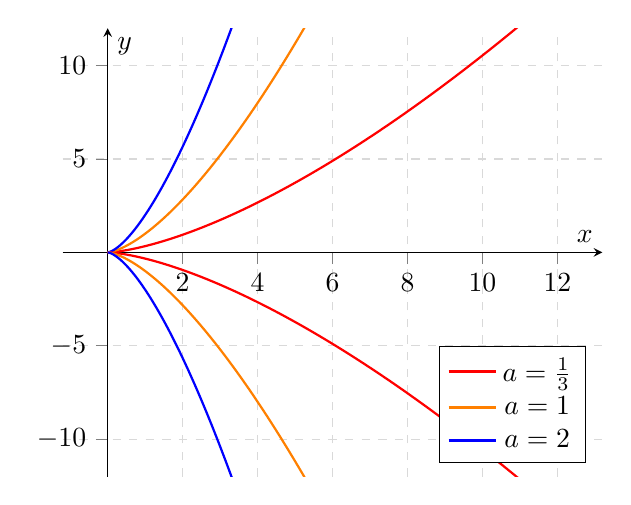
\begin{tikzpicture}
    \begin{axis}[
        legend pos=south east,
        axis x line=middle,
        axis y line=middle,
        grid = major,
        %width=9cm,
        %height=4.5cm,
        grid style={dashed, gray!30},
        xmin= 0,     % start the diagram at this x-coordinate
        xmax= 12,    % end   the diagram at this x-coordinate
        ymin=-10,     % start the diagram at this y-coordinate
        ymax= 10,   % end   the diagram at this y-coordinate
        %axis background/.style={fill=white},
        xlabel=$x$,
        ylabel=$y$,
        %xticklabels={-2,-1.6,...,7},
        tick align=outside,
        %minor tick num=-3,
        enlargelimits=true]
      \addplot[domain=0:12, red, thick,samples=500] {1/3*x^1.5}; 
      \addplot[domain=0:12, orange, thick,samples=500] {1*x^1.5}; 
      \addplot[domain=0:12, blue, thick,samples=500] {2*x^1.5}; 

      \addplot[domain=0:12, red, thick,samples=500] {-1/3*x^1.5}; 
      \addplot[domain=0:12, orange, thick,samples=500] {-1*x^1.5}; 
      \addplot[domain=0:12, blue, thick,samples=500] {-2*x^1.5}; 
      \addlegendentry{$a=\frac{1}{3}$}
      \addlegendentry{$a=1$}
      \addlegendentry{$a=2$}
    \end{axis} 
\end{tikzpicture}

                    \label{fig:semicubical-parabola-3d}
                }%
                \label{Neilsche-Parabel}
                \caption{Rechts ist die Neilsche Parabel für verschiedene Parameter $a$.}
            \end{figure}
              Es gilt: $\text{grad}(F) = (-3x^2, 2y)$. Also: $\text{grad}(0,0) = (0,0)$.
              Daher ist Korollar \label{Mannigfaltigkeitskriterium}
              nicht anwendbar, aber $V(F)$ ist trotzdem
              eine 1-dimensionale topologische Mannigfaltigkeit.
    \end{enumerate}
\end{beispiel}

\begin{definition}\xindex{Mannigfaltigkeit!mit Rand}
    Sei $X$ ein Hausdorffraum mit abzählbarer Basis der Topologie.
    $X$ heißt $n$-dimensionale \textbf{Mannigfaltigkeit mit Rand},
    wenn es einen Atlas $(U_i, \varphi_i)$ gibt, wobei $U_i \subseteq X_i$
    offen und $\varphi_i$ ein Homöomorphismus auf eine offene 
    Teilmenge von 
    \[R_{+,0}^n := \Set{(x_1, \dots, x_n) \in \mdr^n | x_m \geq 0}\]
    ist. $R_{+,0}^n$ ist ein \enquote{Halbraum}.
\end{definition}

\begin{figure}[ht]
    \centering
    \subfloat[Halbraum]{
        \documentclass[varwidth=true, border=2pt]{standalone}
\usepackage{tikz}
\usetikzlibrary{patterns}

\begin{document}
    \begin{tikzpicture}
        \draw [white,step=0.5cm, pattern=north east lines] (0,0) rectangle (2,1);
        \draw[very thick] (0,0) -- (2,0);

        \node at (2.4,0.5) {$\stackrel{\sim}{=}$};

    \begin{scope}[shift={(4,0)}]
        \draw[white,pattern=north east lines] ([shift={(180:1cm)}]-0.0,0) arc (180:0:1cm);
        \draw[very thick] (-1,0) -- (1,0);
    \end{scope}
    \end{tikzpicture}
\end{document}

        \label{fig:half-space}
    }%

    \subfloat[Pair of pants]{
        \begin{tikzpicture}[tqft/flow=east]
    \node[tqft/pair of pants,draw,rotate=-180] (a) {};
    \draw (-1.02,-1) ellipse (0.2cm and 0.35cm);
    \draw (-1.02,+1) ellipse (0.2cm and 0.35cm);
    \draw[dashed] (1,0) ellipse (0.175cm and 0.35cm);

    \draw (2.3,0) ellipse (0.7cm and 1.5cm);
    \draw (2.3,+0.5) circle (0.3cm);
    \draw (2.3,-0.5) circle (0.3cm);

    \node at (1.38,0) {$\stackrel{\sim}{=}$};
\end{tikzpicture}

        \label{fig:pair-of-pants}
    }%
    \subfloat[Sphäre mit einem Loch]{
        \documentclass[varwidth=true, border=2pt]{standalone}
\usepackage{tikz}
\usepackage{tqft}

\begin{document}
    \begin{tikzpicture}[tqft/flow=east]
        \draw (0,0) circle (2cm);
        \draw (0,0) ellipse (2cm and 0.35cm);
        \draw[white,fill=white] (0,0.1) ellipse (1.95cm and 0.35cm);
        \draw[dashed] (0,0) ellipse (2cm and 0.35cm);

        \begin{scope}[rotate=45]
            \draw (0.5,1.2) ellipse (0.5cm and 0.4cm);
        \end{scope}

        \node at (2.38,0) {$\stackrel{\sim}{=}$};

        \draw (3.8,0) circle (1cm);
    \end{tikzpicture}
\end{document}

        \label{fig:sphere-with-hole}
    }%
    \label{Mannigfaltigkeiten mit Rand}
    \caption{Beispiele für Mannigfaltigkeiten mit Rand}
\end{figure}

\begin{definition}\xindex{Rand}
    Sei $X$ eine $n$-dimensionale Mannigfaltigkeit mit Rand und
    Atlas $(U_i, \varphi_i)$. Dann heißt 
    \[\partial X := \bigcup_{i\in I} \Set{x \in U_i | \varphi_i (x)_n = 0}\]
    \textbf{Rand} von $X$.
\end{definition}

$\partial X$ ist eine Mannigfaltigkeit der Dimension $n-1$.

\begin{definition}\xindex{Kartenwechsel}\xindex{bergangsfunktion}
    Sei $X$ eine $n$-dimensionale Mannigfaltigkeit mit Atlas
    $(U_i, \varphi_i)_{i \in I}$

    \begin{enumerate}[label=\alph*)]
        \item Für $i, j \in I$ mit $U_i, U_j \neq \emptyset$ heißt
              \begin{align*}
                \varphi_{ij} &:= \varphi_j \circ \varphi_i^{-1}\\
                \varphi_i (U_i \cap U_j) &\rightarrow \varphi_j (U_i \cap U_j)
              \end{align*}
              \textbf{Kartenwechsel} oder \textbf{Übergangsfunktion}.
    \end{enumerate}
\end{definition}

\begin{figure}[htp]
    \centering
    \documentclass[varwidth=true, border=2pt]{standalone}
\usepackage{amsmath,amssymb}% math symbols / fonts
\usepackage{tikz}
\usetikzlibrary{patterns}

\begin{document}
    \begin{tikzpicture}
        \draw (0,0) ellipse (2cm and 1cm);
        \begin{scope}[xshift=-2.2cm,yshift=-2.8cm]
            \draw[->] (0,0) -- (0,1.5);
            \draw[->] (0,0) -- (1.5,0);
            \node at (0.3,0.16) {$\mathbb{R}^n$};
        \end{scope}
        \begin{scope}[xshift=0.4cm,yshift=-2.8cm]
            \draw[->] (0,0) -- (0,1.5);
            \draw[->] (0,0) -- (1.5,0);
            \node at (0.3,0.16) {$\mathbb{R}^n$};
        \end{scope}
        \def\ringa{(-0.3,0) circle (0.5cm)}
        \def\ringb{(+0.3,0) circle (0.5cm)}

        \begin{scope}[even odd rule]
            \clip \ringa;
            \fill[pattern color=red,pattern=north east lines] \ringb;
        \end{scope}

        \begin{scope}[even odd rule,shift={(-0.7,-2)}]
            \clip \ringa;
            \fill[draw=red,pattern color=red,pattern=north east lines] \ringb;
        \end{scope}

        \begin{scope}[even odd rule,shift={(+0.7,-2)}]
            \clip \ringb;
            \fill[draw=red,pattern color=red,pattern=north east lines] \ringa;
        \end{scope}
        \draw \ringa;
        \draw \ringb;

        \node at (-1,0.3) {$U_i$};
        \node at (+1,0.3) {$U_j$};
        \node at (-1.9,-2) {$V_i$};
        \node at (+1.9,-2) {$V_j$};
        \node at (+2.0,0.7) {$X$};

        \path[->] (-0.35,0)  edge [bend angle=10,bend right] node[label={[label distance=0.1cm]210:$\varphi_i$}] {} (-1,-1.5);
        \path[->] (+0.35,0)  edge [bend angle=10,bend left]  node[label={[label distance=0.1cm]-30:$\varphi_j$}] {} (+1,-1.5);

        \draw (-1,-2) circle (0.5cm);
        \draw (+1,-2) circle (0.5cm);

        \draw[->, red, thick] (-0.3,-2) -- (0.3,-2);
    \end{tikzpicture}
\end{document}

    \caption{Kartenwechsel}
    \label{fig:kartenwechsel}
\end{figure}

%%%%%%%%%%%%%%%%%%%%%%%%%%%%%%%%%%%%%%%%%%%%%%%%%%%%%%%%%%%%%%%%%%%%%
% Mitschrieb vom 19.11.2013                                         %
%%%%%%%%%%%%%%%%%%%%%%%%%%%%%%%%%%%%%%%%%%%%%%%%%%%%%%%%%%%%%%%%%%%%%
\section{Differenzierbare Mannigfaltigkeiten}
\begin{definition}
    Sei $X$ eine $n$-dimensionale Mannigfaltigkeit mit Atlas $(U_i, \varphi_i)_{i \in I}$.

    \begin{enumerate}[label=\alph*)]
        \item $X$ heißt \textbf{differenzierbare Mannigfaltigkeit der Klasse $C^k$}\xindex{Mannigfaltigkeit!differenzierbare},
              wenn jede Kartenwechselabbildung $\varphi_{ij},\;i,j \in I$
              $k$-mal stetig differenzierbar ist.
        \item $X$ heißt \textbf{differenzierbare Mannigfaltigkeit}\xindex{Mannigfaltigkeit!glatte},
              wenn $X$ eine differenzierbare Mannigfaltigkeit der
              Klasse $C^\infty$ ist.
    \end{enumerate}
\end{definition}

\begin{definition}
    Sei $X$ eine differenzierbare Mannigfaltigkeit der Klasse $C^k$ 
    ($k \in \mdn \cup \Set{\infty}$) mit Atlas $(U_i, \varphi_i)_{i \in I}$.

    \begin{enumerate}[label=\alph*)]
        \item Eine Karte $(U, \varphi)$ auf $X$ heißt \textbf{verträglich}\xindex{verträglich}
              mit $\atlas$, wenn alle Kartenwechsel $\varphi \circ \varphi_i^{-1}$
              und $\varphi_i \circ \varphi^{-1}$ ($i \in I$ mit $U_i \cap U \neq \emptyset$)
              differenzierbar von Klasse $C^k$ sind.
        \item Die Menge aller mit $\atlas$ verträglichen Karten auf 
              $X$ bildet einen maximalen Atlas von Klasse $C^k$. Er
              heißt \textbf{$C^k$-Struktur}\xindex{$C^k$-Struktur} auf $X$.
            
              Eine $C^\infty$-Struktur heißt auch \textbf{differenzierbare Struktur}\xindex{Struktur!differenzierbare}
              auf $X$.
    \end{enumerate}
\end{definition}

\begin{bemerkung}
    Für $n \geq 4$ gibt es auf $S^n$ mehrere verschiedene differenzierbare
    Strukturen, die sog. \enquote{exotische Sphären}\xindex{Sphäre!exotische}.
\end{bemerkung}

\begin{definition}
    Seien $X, Y$ differenzierbare Mannigfaltigkeiten der Dimension
    $n$ bzw. $m$, $x \in X$.

    \begin{enumerate}[label=\alph*),ref=\theplaindefinition.\alph*]
        \item Eine stetige Abbildung $f:X \rightarrow Y$ heißt\label{def:stetigeAbbildungDiffbar}
              \textbf{differenzierbar}\xindex{Abbildung!differenzierbare}
              in $X$ (von Klasse $C^k$),
              wenn es Karten $(U, \varphi)$ von $X$ mit
              $x \in U$ und $(V, \psi)$ von $Y$ mit $f(U) \subseteq V$
              gibt, sodass $\psi \circ f \circ \varphi^{-1}$ stetig
              differenzierbar von Klasse $C^k$ in $\varphi(x)$ ist.
        \item $f$ heißt \textbf{differenzierbar}\todo{stimmt das so?}
              (von Klasse $C^k$), wenn $f$ in jedem $x \in X$ 
              differenzierbar ist.
        \item $f$ heißt \textbf{Diffieomorphismus}\xindex{Diffieomorphismus},
              wenn $f$ differenzierbar von Klasse $C^\infty$ ist und
              es eine differenzierbare Abbildung $g: Y \rightarrow X$
              von Klasse $C^\infty$ gibt mit $g \circ f = \text{id}_X$
              und $f \circ g = \text{id}_Y$.
    \end{enumerate}
\end{definition}

\begin{korollar}
    Die Bedingung in Definition \ref{def:stetigeAbbildungDiffbar} hängt nicht
    von den gewählten Karten ab.
\end{korollar}

\begin{beweis}
    Seien $(U', \varphi')$ und $(V', \psi')$ Karten von $X$ bzw. $Y$
    um $x$ bzw. $f(x)$ mit $f(U') \subseteq V'$.

    \begin{align*}
        \Rightarrow &\psi' \circ f \circ (\varphi')^{-1}\\
                  = &\psi' \circ ( \psi^{-1} \circ \psi) \circ f \circ (\varphi^{-1} \circ \varphi ) \circ (\varphi')^{-1}
    \end{align*}

    ist genau dann differenzierbar, wenn $\psi \circ f \circ \varphi^{-1}$
    differenzierbar ist.
\end{beweis}

\begin{beispiel}
    $f: \mdr \rightarrow \mdr, \;\;\; x \mapsto x^3$ ist kein
    Diffieomorphismis, aber Homöomorphismus, da mit $g(x) := \sqrt[3]{x}$
    gilt: $f \circ g = \text{id}_\mdr, \;\;\; g \circ f = \text{id}_\text{\mdr}$
\end{beispiel}

\begin{bemerkung}
    Sei $X$ eine glatte Mannigfaltigkeit. Dann ist
    \[\text{Diffeo}(X) := \Set{f:X \rightarrow X | f \text{ ist Diffeomorphismus}}\]
    eine Untergruppe von $\text{Homöo}(X)$.
\end{bemerkung}

\begin{definition}
    Eine Teilmenge $S \subseteq \mdr^3$ heißt \textbf{reguläre Fläche}\xindex{Fläche!reguläre},
    wenn es für jedes $s \in S$ eine Umgebung $V$ von $\sin{\mdr^3}$
    eine offene Teilmenge $F: U \rightarrow V \cap S$ gibt, sodass
    die Jacobi-Matrix $J_F(u)$ für alle $u \in U$ Rang 2 hat.

    $F$ heißt (lokale) reguläre Parametrisierung von $S$.

    \begin{align*}
        F(u,v) &= \left (x(u,v), y(u,v), z(u,v) \right )\\
        J_F(u,v) &= \begin{pmatrix}
            \frac{\partial x}{\partial u} (p) & \frac{\partial x}{\partial v} (p)\\
            \frac{\partial y}{\partial u} (p) & \frac{\partial y}{\partial v} (p)\\
            \frac{\partial z}{\partial u} (p) & \frac{\partial z}{\partial v} (p)
        \end{pmatrix}
    \end{align*}
\end{definition}

\begin{beispiel}
    \begin{enumerate}[label=\arabic*)]
        \item Rotationsflächen: Sei $r:\mdr \rightarrow \mdr_{> 0}$
              eine differenzierbare Funktion.

              $F: \mdr^2 \rightarrow \mdr^3 \;\;\; (u,v) \mapsto (r(u) \cos (u), r(v) \sin(u), v)$


            \begin{figure}
                \centering
                \subfloat[Kugelkooridnaten]{
                    \includegraphics[width=0.4\linewidth, keepaspectratio]{figures/spherical-coordinates.pdf}
                    \label{fig:spherical-coordinates}
                }%
                \subfloat[Rotationskörper]{
                    \pgfplotsset{
    colormap={whitered}{
        color(0cm)=(white);
        color(1cm)=(orange!75!red)
    }
    %colormap={color}{color(0cm)=(white); color(1cm)=(blue)}
}
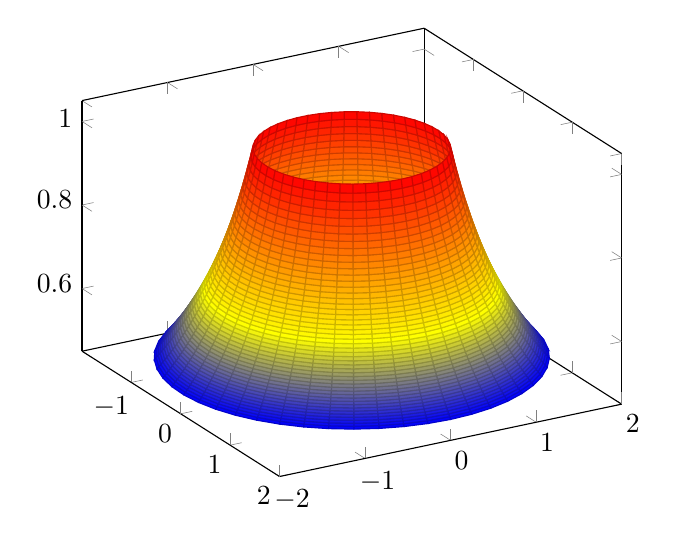
\begin{tikzpicture}
 \begin{axis}[view={60}{30}]
  \addplot3[surf,
  samples=50,
  domain=1:2,y domain=0:2*pi,
  z buffer=sort]
  %({(2 + tan(deg(y)))*cos((deg(x)))}, {(2 + cos(x)) * sin(x)}, {x});
  ({x * cos(deg(y))}, {x * sin(deg(y))}, {1/x});
 \end{axis}
\end{tikzpicture}

                    \label{fig:solid-of-revolution}
                }%

                \subfloat[Sinus und Cosinus]{
                    \includegraphics[width=0.8\linewidth, keepaspectratio]{figures/sin-cos.pdf}
                    \label{fig:sin-cos}
                }%
                \label{Formen}
                %\caption{}
            \end{figure}

            \[J_F(u,v) = 
            \begin{pmatrix}
                -r(v) \sin u & r'(v) \cos u\\
                r(v) \cos u  & r'(v) \sin u\\
                 0           & 1
            \end{pmatrix}\]
            hat Rang 2 für alle $(u,v) \in \mdr^2$.
        \item Kugelkoordinaten: $F: \mdr^2 \rightarrow \mdr^3, \;\;\; (u, v) \mapsto (R \cos v \cos u, R \cos v \sin u, R \sin v)$
              $F(u,v) \in S_R^2$, denn 
                \begin{align*}
                    & R^2 \cos^2(v) \cos^2(u) + R^2 \cos^2(v) \sin^2(u) + R^2 \sin^2(v)\\
                    =& R^2 (\cos^2(v) \cos^2(u) + \cos^2(v) \sin^2(u) + \sin^2(v))\\
                    =& R^2 \left (\cos^2(v) (\cos^2(u) + \sin^2(u)) + \sin^2(v) \right)\\
                    =& R^2 \left (\cos^2(v) + \sin^2(v) \right)\\
                    =&R^2
                \end{align*}

                Die Jacobi-Matrix
                \[J_F(u,v) = 
                \begin{pmatrix}
                    -R \cos v \sin u & -R \sin v \cos u\\
                    R \cos v \cos u  & -R \sin v \sin u\\
                    0                & R \cos v
                \end{pmatrix}\]
                hat Rang 2 für $\cos v \neq 0$. In $N$ und $S$ ist
                $\cos v = 0$.
    \end{enumerate}
\end{beispiel}

% Die Übungsaufgaben sollen ganz am Ende des Kapitels sein.
\clearpage
\section*{Übungsaufgaben}
\addcontentsline{toc}{section}{Übungsaufgaben}

\begin{aufgabe}[Zusammenhang]\label{ub4:aufg1}
    \begin{enumerate}[label=(\alph*)]
        \item Beweisen Sie, dass eine topologische Mannigfaltigkeit
              genau dann wegzusammenhängend ist, wenn sie zusammenhängend
              ist
        \item Betrachten Sie nun wie in Beispiel~\ref{bsp:mannigfaltigkeit8}
              den Raum $X:= (\mdr \setminus \Set{0}) \cup \Set{0_1, 0_2}$
              versehen mit der dort definierten Topologie. Ist $X$
              wegzusammenhängend?
    \end{enumerate}
\end{aufgabe}

